%!TEX root = ../dokumentation.tex

\chapter{Implementierung des Tools}

\section{Grundstruktur der Applikation}

Die Grundstruktur der Applikation basiert auf zwei im MATLAB App Designer erstellten Applikationen. Der Hauptapplikation, welche das Aufrufen einzelner Funktionalität ermöglicht, sowie den Graphen der erstellen Visualisierungen darstellt, und die Applikation zur Konfiguration der Samples, welche parallel zur Hauptapplikation als Pop-Up geöffnet werden kann, jedoch nicht ohne diese verwendbar ist. Als dritte Struktur wurde die sogenannte WithSamplesParser-Klasse erstellt, welche alle Funktionalitäten bezüglich der Messdatenverarbeitung und Darstellung enthält. Dazu gehören das Auslösen, Umstrukturieren auf ein passendes Format der Messdaten sowie das Erstellen eines Graphen mit der passenden Konfiguration. Diese Funktionen werden dabei ebenfalls aus der Hauptapplikationen gestartet und benötigen diese deshalb auch also Grundlage.

\begin{figure}[!htbp]
	\centering
	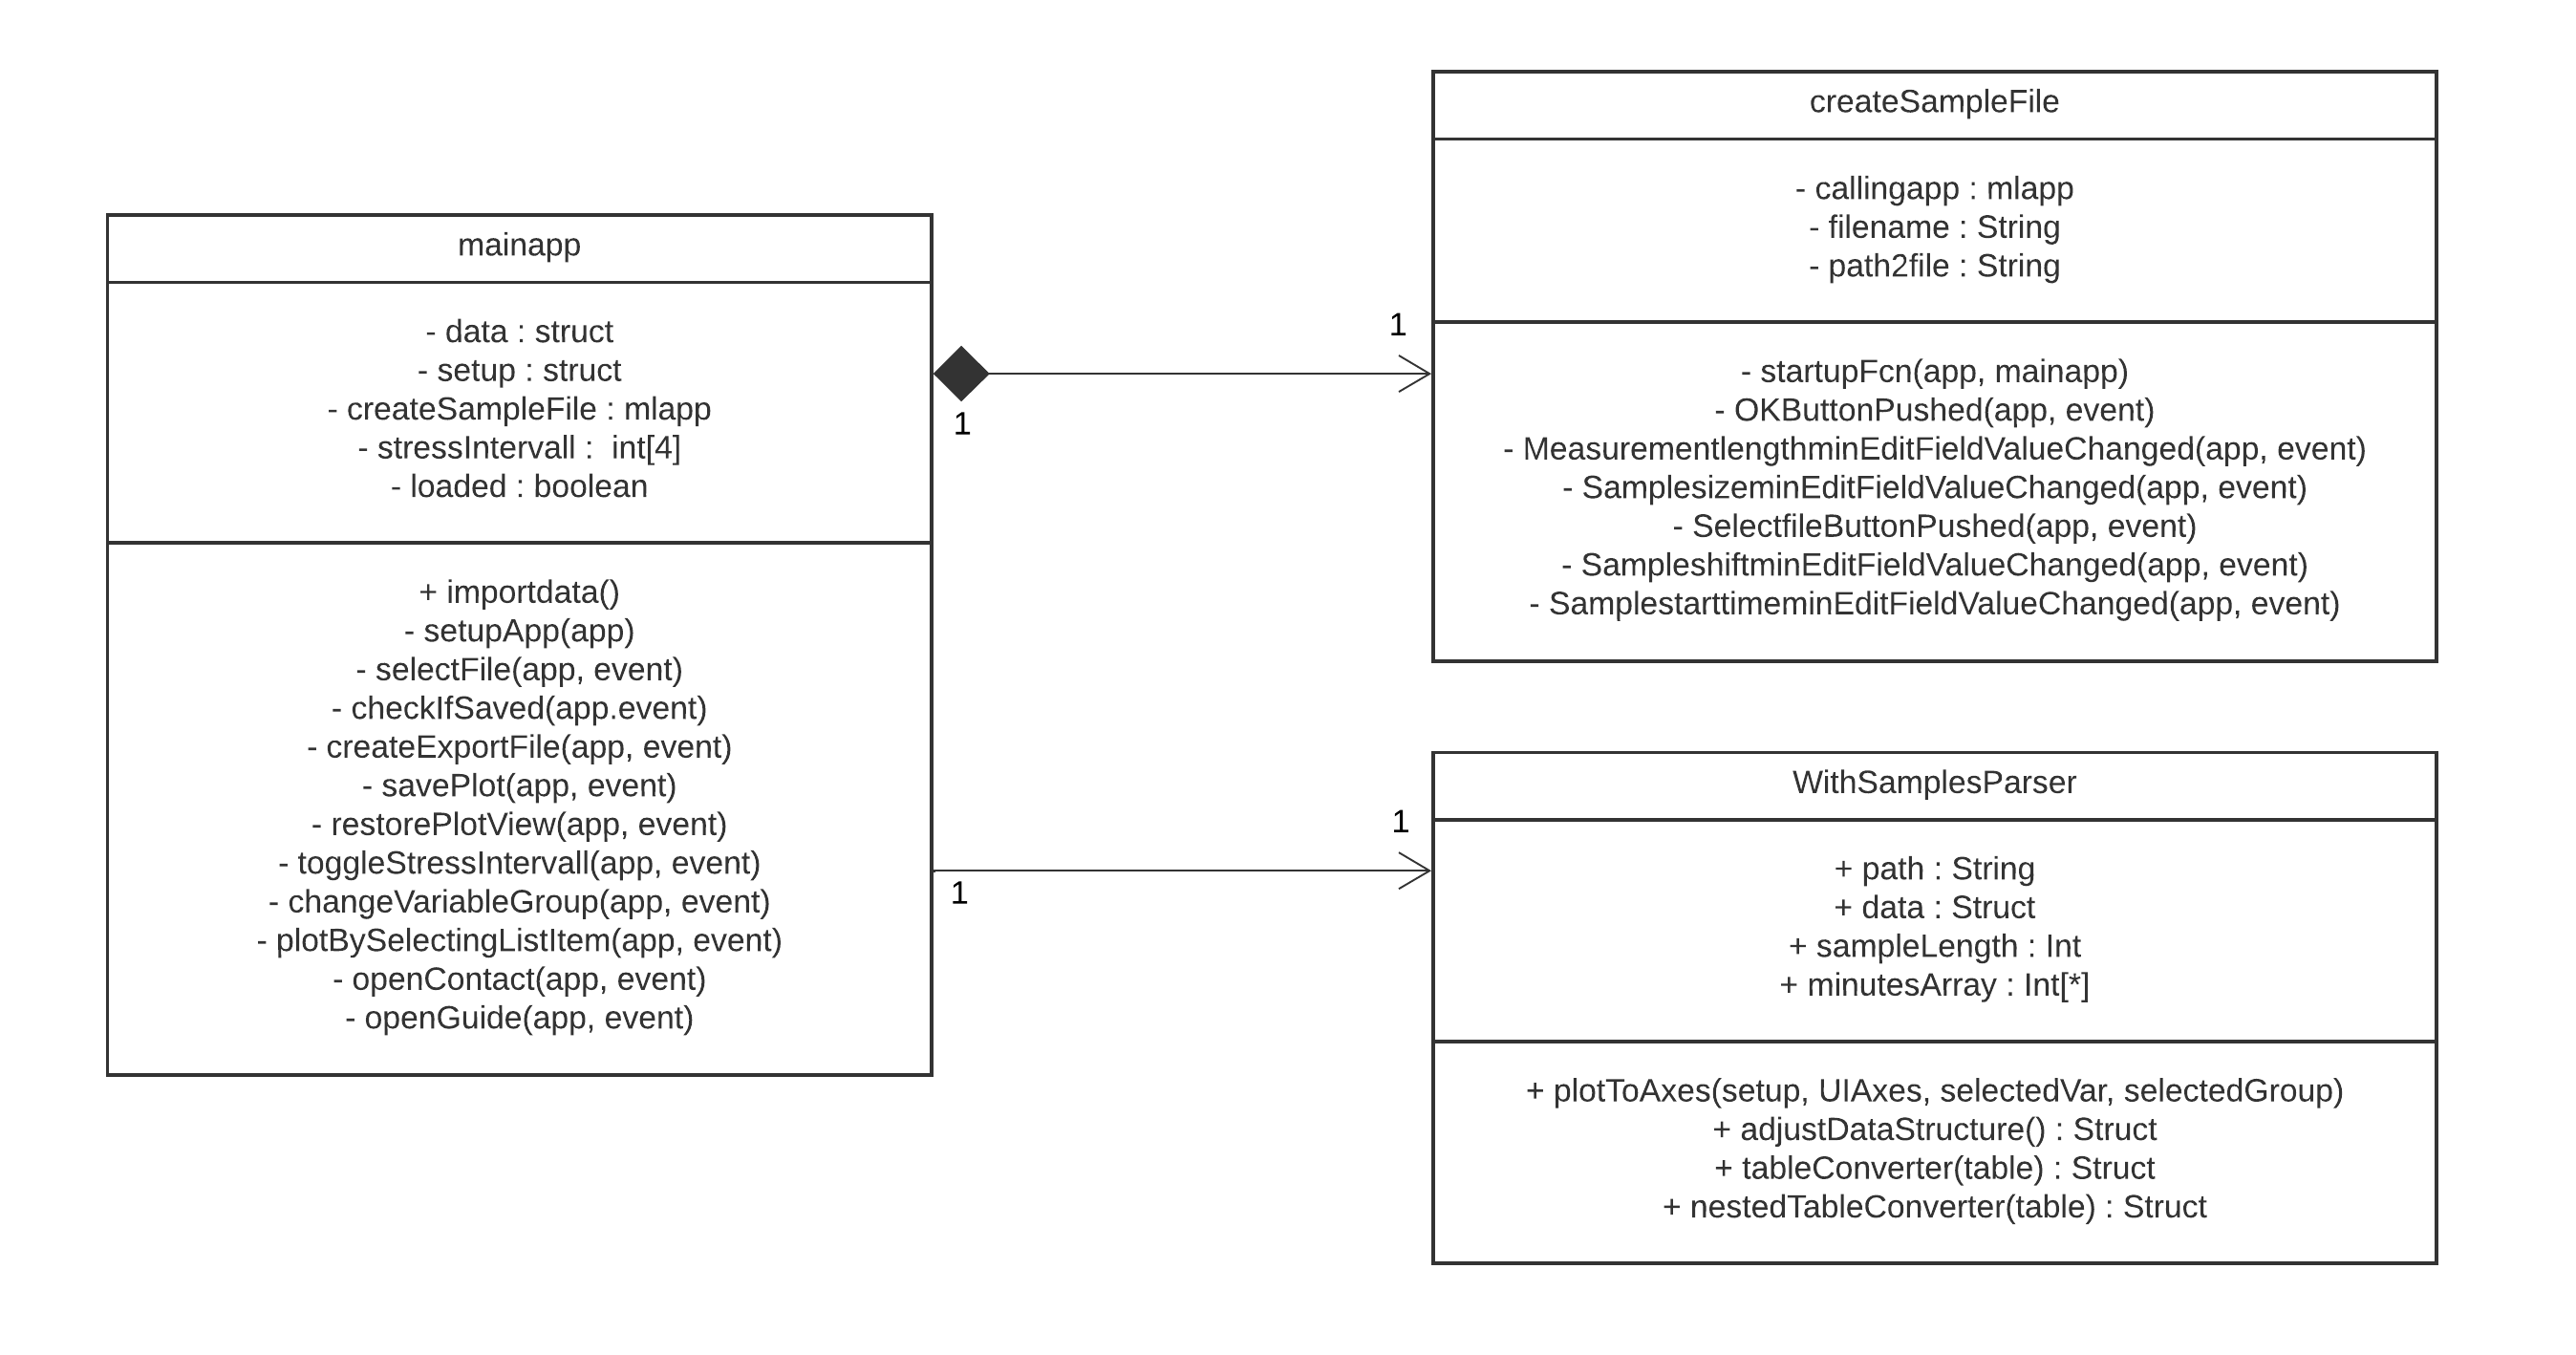
\includegraphics[width=1\linewidth]{klassendiagramm}
	\caption{Klassendiagramm der fertigen Applikation}
	\label{fig:klassendiagramm}
\end{figure}

\section{Erstellung der Samples}

\section{Visualisierung der Daten}

\subsection{Datenstruktur}

\subsection{Plot-Funktion}

\subsection{Zusätzliche Funktionen}